\section{TEST A-CLUS BASE}

Durante la fase di testing, sono stati analizzati diversi scenari critici per validare la robustezza dell'applicazione:

\substection{Gestione di tabelle inesistenti}

\begin{figure}[h!]
    \centering
    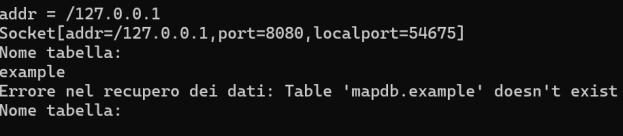
\includegraphics[width=\textwidth]{images/errore_tabella.png.png}
\end{figure}

Quando viene specificato un identificativo di tabella non presente nel database, il sistema visualizza un appropriato messaggio diagnostico e offre all'utente la possibilità di inserire una denominazione alternativa.


\subsection{Validazione delle selezioni di menù}

\begin{figure}[h!]
    \centering
    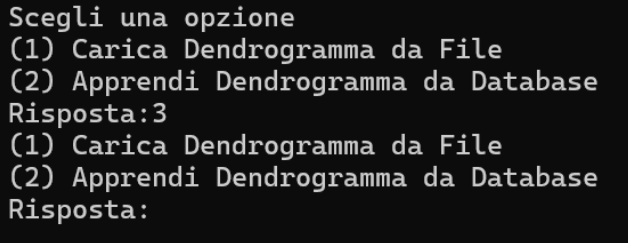
\includegraphics[width=\textwidth]{images/errore_men.png}
\end{figure}

L'inserimento di valori non conformi alle opzioni disponibili (diversi da 1 o 2) viene intercettato, consentendo all'utente di ripetere la selezione senza interruzioni del flusso operativo.

\subsubsection{Controllo sull'esistenza degli archivi} 
\begin{figure}[h!]
    \centering
    \includegraphics[width=\textwidth]{images/controllo_archivi.png}
\end{figure}
Nel caso di caricamento di un dendrogramma precedentemente salvato, il sistema verifica l'esistenza dell'archivio specificato. In caso negativo, viene presentata una notifica e l'applicazione termina la sessione.

\subsubsection{Validazione parametri di profondità} 
    \begin{figure}[h!]
        \centering
        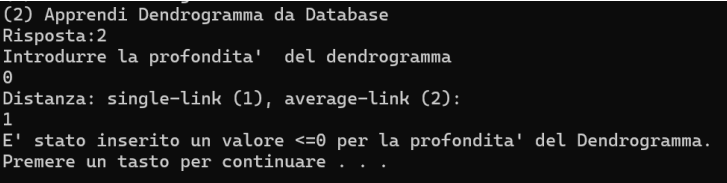
\includegraphics[width=\textwidth]{images/0_valore_errato.png}
    \end{figure}

    \begin{figure}[h!]
        \centering
        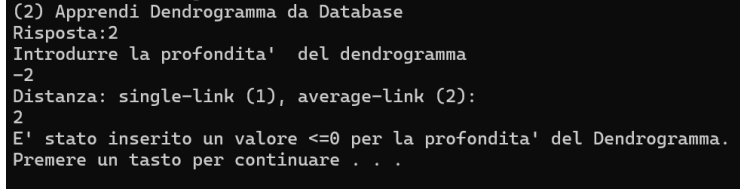
\includegraphics[width=\textwidth]{images/-2_valore_errato.png}
    \end{figure}

    L'inserimento di valori non ammissibili per il parametro di profondità (zero o negativi) viene rilevato dal sistema che, pur proseguendo con la richiesta del metodo di calcolo, interromperà l'elaborazione notificando l'anomalia.

\subsubsection{Controllo selezioni metodologiche} 
    
\begin{figure}[h!]
        \centering
        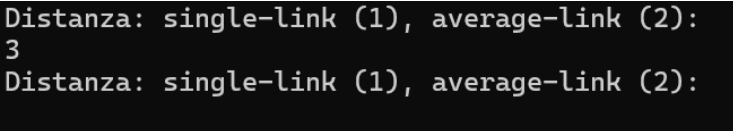
\includegraphics[width=\textwidth]{images/controllo_metodologie.png}
    \end{figure}
    L'inserimento di opzioni non valide per la selezione della metodologia di calcolo delle distanze viene gestito permettendo all'utente di riformulare la propria scelta.

\subsubsection{Verifica di compatibilità dimensionale} 
    \begin{figure}[h!]
        \centering
        \includegraphics[width=\textwidth]{images/compatibilità_dimensionale.png}
    \end{figure}
    Il sistema controlla la congruenza tra la cardinalità degli esempi nella tabella corrente e quella memorizzata nell'oggetto serializzato. In caso di incongruenza, viene visualizzato un messaggio esplicativo e l'esecuzione viene terminata.

\subsection{Gestione connettività client-server}
\begin{figure}[h!]
    \centering
    \includegraphics[width=\textwidth]{images/connettività_clientserver.png.png}
\end{figure}
L'avvio del client in assenza del componente server attivo genera un tentativo di connessione all'indirizzo locale (127.0.0.1) che, non trovando un endpoint disponibile, risulta in un rifiuto della connessione con relativa notifica.

\subsubsection{Elaborazione su dataset vuoti} 
    \begin{figure}[h!]
        \centering
        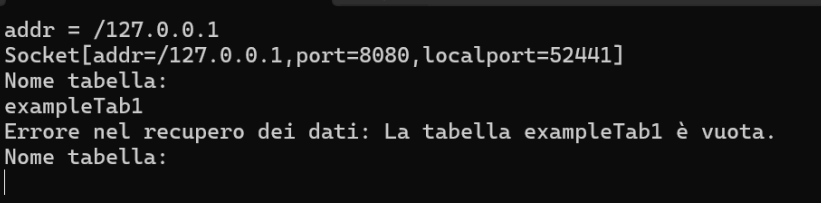
\includegraphics[width=\textwidth]{images/dataset_vuoti.png}
    \end{figure}

Quando l'utente tenta di eseguire un'analisi di clustering su una tabella priva di contenuti, il sistema identifica la condizione e fornisce un'appropriata segnalazione.


\section{Cambiamenti}

\subsection{Cambiamenti Motivati nella Versione Base Rispetto i Requisiti del Progetto}

\begin{enumerate}
    \item \textbf{Metodo getLength() in ClusterSet / Metodo getLevel0Length() in HierarchicalClusterMiner:}
    \begin{itemize}
        \item \textbf{Descrizione getLength():} Questo metodo restituisce la lunghezza dell'array C in ClusterSet.
        \item \textbf{Descrizione getLevel0Length():} Questo metodo restituisce la lunghezza del set di cluster al livello 0 del dendrogramma.
        \item \textbf{Motivazione:} Abbiamo aggiunto questi metodi per ottenere il numero di elementi presenti nel ClusterSet al livello 0 del dendrogramma e per passare tale informazione al metodo loadDendrogramFromFile() in ServerOneClient. Questo permette di verificare qui che il numero di esempi nella tabella scelta non sia minore del numero di esempi con cui è stato salvato il dendrogramma precedentemente.
    \end{itemize}
    
    \item \textbf{Metodo getDepth() in HierarchicalClusterMiner:}
    \begin{itemize}
        \item \textbf{Descrizione getDepth():} Questo metodo restituisce la profondità del dendrogramma in HierarchicalClusterMiner.
        \item \textbf{Motivazione:} Abbiamo aggiunto questo metodo per verificare nel metodo loadDendrogramFromFile() in ServerOneClient che la profondità del dendrogramma caricato da file non sia maggiore del numero di esempi nella tabella scelta dall'utente.
    \end{itemize}
\end{enumerate}

\subsection{Cambiamenti Motivati nella Versione Estesa Rispetto alla Base}

\begin{enumerate}
    \item \textbf{Rimossa responsabilità gestione macchina a stati nel server.}\\
    Nella versione base del programma, il metodo run di ServerOneClient memorizzava l'oggetto Data, che rappresentava la tabella contenente il dataset scelto dall'utente. Questo oggetto era creato alla prima richiesta dal client, nel momento in cui l'utente specificava quale tabella del database utilizzare. I dati erano poi conservati all'interno del thread avviato per ciascuna connessione tra client e server, e mantenuti attivi grazie a un ciclo while true, che proseguiva fino alla disconnessione del client.
    
    Nella versione estesa, invece, il client gestisce gli aggiornamenti (Updates) inviati dall'API di Telegram, che contengono i messaggi degli utenti diretti al bot. Teoricamente, il server della versione base potrebbe essere compatibile con il client della versione estesa, poiché è progettato per gestire connessioni multiple tramite multithreading: ogni aggiornamento del bot potrebbe quindi attivare un thread separato del server, avviando una nuova connessione Socket.
    
    Tuttavia, questa soluzione è adatta solo se la connessione socket può rimanere aperta a lungo. Se, per esempio, un utente inviasse un messaggio ora e il successivo solo una settimana dopo, mantenere la connessione aperta risulterebbe inefficiente e costoso, poiché l'unico scopo sarebbe mantenere vivo l'oggetto Data nel thread.
    
    Per questa ragione e per garantire al server una struttura generica, capace di interfacciarsi con client di natura diversa, abbiamo deciso di spostare l'oggetto Data nel client esteso, insieme ad altre informazioni necessarie per la gestione degli stati. Ad esempio, in futuro potrebbero esistere sia un client web sia un client bot Telegram. Supponiamo che un utente esegua due clustering uno sulla versione web e una sulla versione bot Telegram; mantenere tutti i dati di stato sul server limiterebbe la possibilità di separare l'interazione su dispositivi diversi, oltre a imporre uno schema fisso basato sulla macchina a stati anche per i client che non lo necessitano. Un client senza macchina a stati potrebbe, ad esempio, essere una versione web in cui le operazioni ``Carica tabella'', ``Profondità'', ``Distanza'' e ``Clustering'' sono eseguite in un'unica richiesta, senza passare attraverso stati successivi.
    
    Nel nuovo client quando riceve un aggiornamento da parte di un nuovo utente, crea un record nel dizionario memorizzando come chiave l'ID Telegram dell'utente e come valore un'istanza della classe StateContext, che gestisce la macchina a stati. Quando un utente invia un messaggio e la sua chiave è già presente nel dizionario, il sistema esegue le operazioni sul StateContext già esistente per quell'utente. StateContext è responsabile della gestione della macchina a stati e contiene uno Stack di stati, che memorizza la cronologia degli stati attraversati dall'utente, più l'ultimo stato attivo in cui applicare gli aggiornamenti. Inoltre, StateContext include una classe Dati che funge da aggregatore di vari dati condivisi tra gli stati e include anche l'oggetto Data (dataset) originale della versione base del server. In questo modo, il sistema può gestire la persistenza e la transizione degli stati per ciascun utente, senza dover mantenere una connessione server-client attiva per tempi prolungati.
    
    La classe StateContext contiene i seguenti attributi di istanza:
    \begin{itemize}
        \item \textbf{Stack<State> StateHistory:} rappresenta la cronologia degli stati attraversati dall'utente. Di default, lo stack contiene lo stato iniziale passato nel costruttore e viene poi popolato aggiungendo ogni nuovo stato tramite operazioni di push. Questo approccio facilita il rollback degli stati. Ad esempio, se l'utente è nello stato 3 e lo stack contiene gli stati [3, 2, 1], un rollback eseguirà un pop dello stato 3, riportando automaticamente l'utente allo stato 2, senza la necessità di gestire manualmente ogni singolo caso di retrocessione.
    \end{itemize}
    
    Ogni stato ha la proprietà allowBack. Se impostata su false (valore di default), consente il rollback dallo stato corrente. Se invece è impostata su true, non è possibile tornare indietro da quello stato. Questo comportamento è stato applicato allo stato iniziale, poiché non è consentito fare rollback una volta entrati nello stato di avvio. Ad esempio, gli stati Clustering e ShowSavedClustering offrono opzioni per tornare allo stato principale (ossia Start), ma una volta raggiunto lo stato Start, il rollback non è consentito poiché segna l'inizio di una nuova iterazione.
    
    Ogni stato è suddiviso in due fasi di operazione:
    \begin{itemize}
        \item \textbf{Pre-Operation:} viene eseguita una sola volta quando lo stato viene creato o resettato. Nel flusso di lavoro attuale, ogni stato fornisce all'utente una serie di operazioni da eseguire, attende la risposta dell'utente e la valida. La fase di preOperation corrisponde all'operazione di chiedere all'utente cosa desidera fare.
        \item \textbf{Post-Operation:} valida la risposta dell'utente e gestisce le transizioni verso altri stati. Passando StateContext come parametro al metodo postOperation, è possibile richiamare il metodo changeState per indicare il nuovo stato da eseguire. Una volta cambiato lo stato, viene eseguita automaticamente la preOperation del nuovo stato, permettendo al sistema di rispondere immediatamente all'utente con il nuovo set di operazioni disponibili per quello stato.
    \end{itemize}
    
    Durante l'esecuzione di una delle due operazioni possono verificarsi errori dovuti a input non validi, dati incorretti o problemi nelle risposte socket. Il comportamento in caso di errore varia in base alla fase dell'operazione:
    \begin{itemize}
        \item \textbf{Pre-Operation:} un errore in questa fase causa un rollback automatico allo stato precedente. Ad esempio, nella fase di pre-operazione del Clustering, può verificarsi un errore se l'utente sceglie un nome per il file di salvataggio del clustering che esiste già dallo stato precedente. In tal caso, il blocco catch esegue un rollback allo stato precedente (con apposito log d'errore), ovvero lo stato ChooseName della post-operazione, permettendo all'utente di inserire un nuovo nome per il file di salvataggio.
        \item \textbf{Post-Operation:} in questa fase, un eventuale errore non altera il flusso del programma, ma comporta la ripetizione della post-operazione. Ad esempio, nel metodo ChooseDepth, la post-operazione convalida la profondità scelta dall'utente; se questa profondità non è valida o fuori range, viene generata un'eccezione che porta al riavvio della post-operazione (con apposito log d'errore), consentendo all'utente di inserire una nuova profondità valida.
    \end{itemize}
\end{enumerate}

\end{document}